% appendix-main.tex

% Use the ACM large 1-column format class from your template directory
\documentclass[acmlarge]{template/column-format-template/acmart}

% Set up any additional package imports here
\usepackage{graphicx}     % For including graphics
\usepackage{amsmath}      % For advanced math formatting
\usepackage{algorithm}    % For algorithm pseudocode
\usepackage{algorithmic}  % For algorithm pseudocode
\usepackage{booktabs}     % For professional tables
\usepackage{listings}     % For code listings
\usepackage{subcaption}   % For subfigures
\usepackage{url}          % For URLs in bibliography
\usepackage{titlesec}     % For custom formatting
\usepackage{xcolor}       % For colors
\usepackage{listings}     % For code snippets

% Custom settings for listings
\lstset{
    language=Python,                    % Sets the programming language for syntax highlighting
    basicstyle=\footnotesize\ttfamily,  % Sets the font style and size for the code
    keywordstyle=\color{blue},          % Style applied to keywords (e.g., "def", "import")
    commentstyle=\color{gray},          % Style applied to comments (e.g., lines starting with "#")
    stringstyle=\color{red},            % Style applied to strings (e.g., text within quotes)
    linewidth=0.95\linewidth,           % Code block occupies 80% of text width
    xleftmargin=-30pt,                  % Moves the listing 20pt closer to the left margin
    xrightmargin=5pt,                   % Optional: Adds extra padding on the right
    breaklines=true,                    % Automatically breaks long lines to fit within the page width
    captionpos=b,                       % Places the caption below the code block
    abovecaptionskip=5pt,               % Adjusts the space above the caption to 5pt
    belowcaptionskip=8pt,               % Adjusts the space below the caption to 8pt
}

% Remove ACM-specific references and permissions
\setcopyright{none} % Disable copyright
\makeatletter
\@printpermissionfalse
\@printcopyrightfalse
\@acmownedfalse
\makeatother

% Remove ACM reference format
\settopmatter{printacmref=false}
\renewcommand\footnotetextcopyrightpermission[1]{}

% Optional: Plain page style
\pagestyle{plain}

\begin{document}

% Title
\title{SSH Shell Attacks - Appendix}

% Define authors and their affiliations
\author{Andrea Botticella}
\authornote{The authors collaborated closely in developing this project.}
\email{andrea.botticella@studenti.polito.it}
\affiliation{%
  \institution{Politecnico di Torino}
  \city{Turin}
  \country{Italy}
}

\author{Elia Innocenti}
\authornotemark[1]
\email{elia.innocenti@studenti.polito.it}
\affiliation{%
  \institution{Politecnico di Torino}
  \city{Turin}
  \country{Italy}
}

\author{Renato Mignone}
\authornotemark[1]
\email{renato.mignone@studenti.polito.it}
\affiliation{%
  \institution{Politecnico di Torino}
  \city{Turin}
  \country{Italy}
}

\author{Simone Romano}
\authornotemark[1]
\email{simone.romano2@studenti.polito.it}
\affiliation{%
  \institution{Politecnico di Torino}
  \city{Turin}
  \country{Italy}
}

% Short author list for page headers
\renewcommand{\shortauthors}{Botticella, Innocenti, Mignone, and Romano}

\maketitle

\vspace{-0.3cm}

% Table of Contents
\setcounter{tocdepth}{1}
\tableofcontents

\appendix

% Include the appendix sections
% 03-data-exploration-and-preprocessing-appendix.tex

\vspace{-1.25cm}

% Section Title
\section{DATA EXPLORATION AND PRE-PROCESSING}

    % Main Content
    
% 04-supervised-learning-classification-appendix.tex

% Section Title
\section{SUPERVISED LEARNING - CLASSIFICATION}

    % Main Content

    \subsection{Logistic Regression}

        In this section, we detail the steps and results obtained from using the Logistic Regression model during the supervised learning phase of the project. Logistic Regression served as a baseline model to provide an initial understanding of the classification problem. Despite its simplicity, it offered valuable insights into the multi-label classification task.

        \subsubsection{Model Training \\}

            The Logistic Regression model was trained using its default configuration. Specifically, the \texttt{lbfgs} solver was utilized with a regularization parameter \( C = 1 \). The training process aimed to identify potential overfitting or underfitting issues and establish baseline performance metrics.

                \begin{lstlisting}[caption={Train Logistic Regression model}, label={lst:logistic_regression_train}]
                        # Initialize and train Logistic Regression model
                        model = LogisticRegression(max_iter=1000, random_state=42)
                        model.fit(X_train_tfidf, y_train_binary)
                \end{lstlisting}

            The dataset was preprocessed using the TF-IDF representation of the session texts, which assigned weights to words based on their frequency and relevance within the dataset. Multi-label binary encoding was applied to the `Set\_Fingerprint` column to ensure compatibility with the model.

        \subsubsection{Evaluation Metrics \\}

            The Logistic Regression model was evaluated using standard classification metrics, including weighted F1-scores, precision, and recall. The evaluation metrics highlighted the strengths and weaknesses of the model in handling imbalanced classes. 

                \begin{lstlisting}[caption={Generate classification report}, label={lst:logistic_regression_eval}]
                        # Generate classification report
                        from sklearn.metrics import classification_report
                        report = classification_report(y_test_binary, y_pred, zero_division=0)
                        print(report)
                \end{lstlisting}

            The confusion matrix provided a breakdown of true positives, false positives, false negatives, and true negatives for each intent. Figure~\ref{fig:logistic_cm} shows the confusion matrix for the Logistic Regression model.

            \begin{figure}[H]
                \centering
                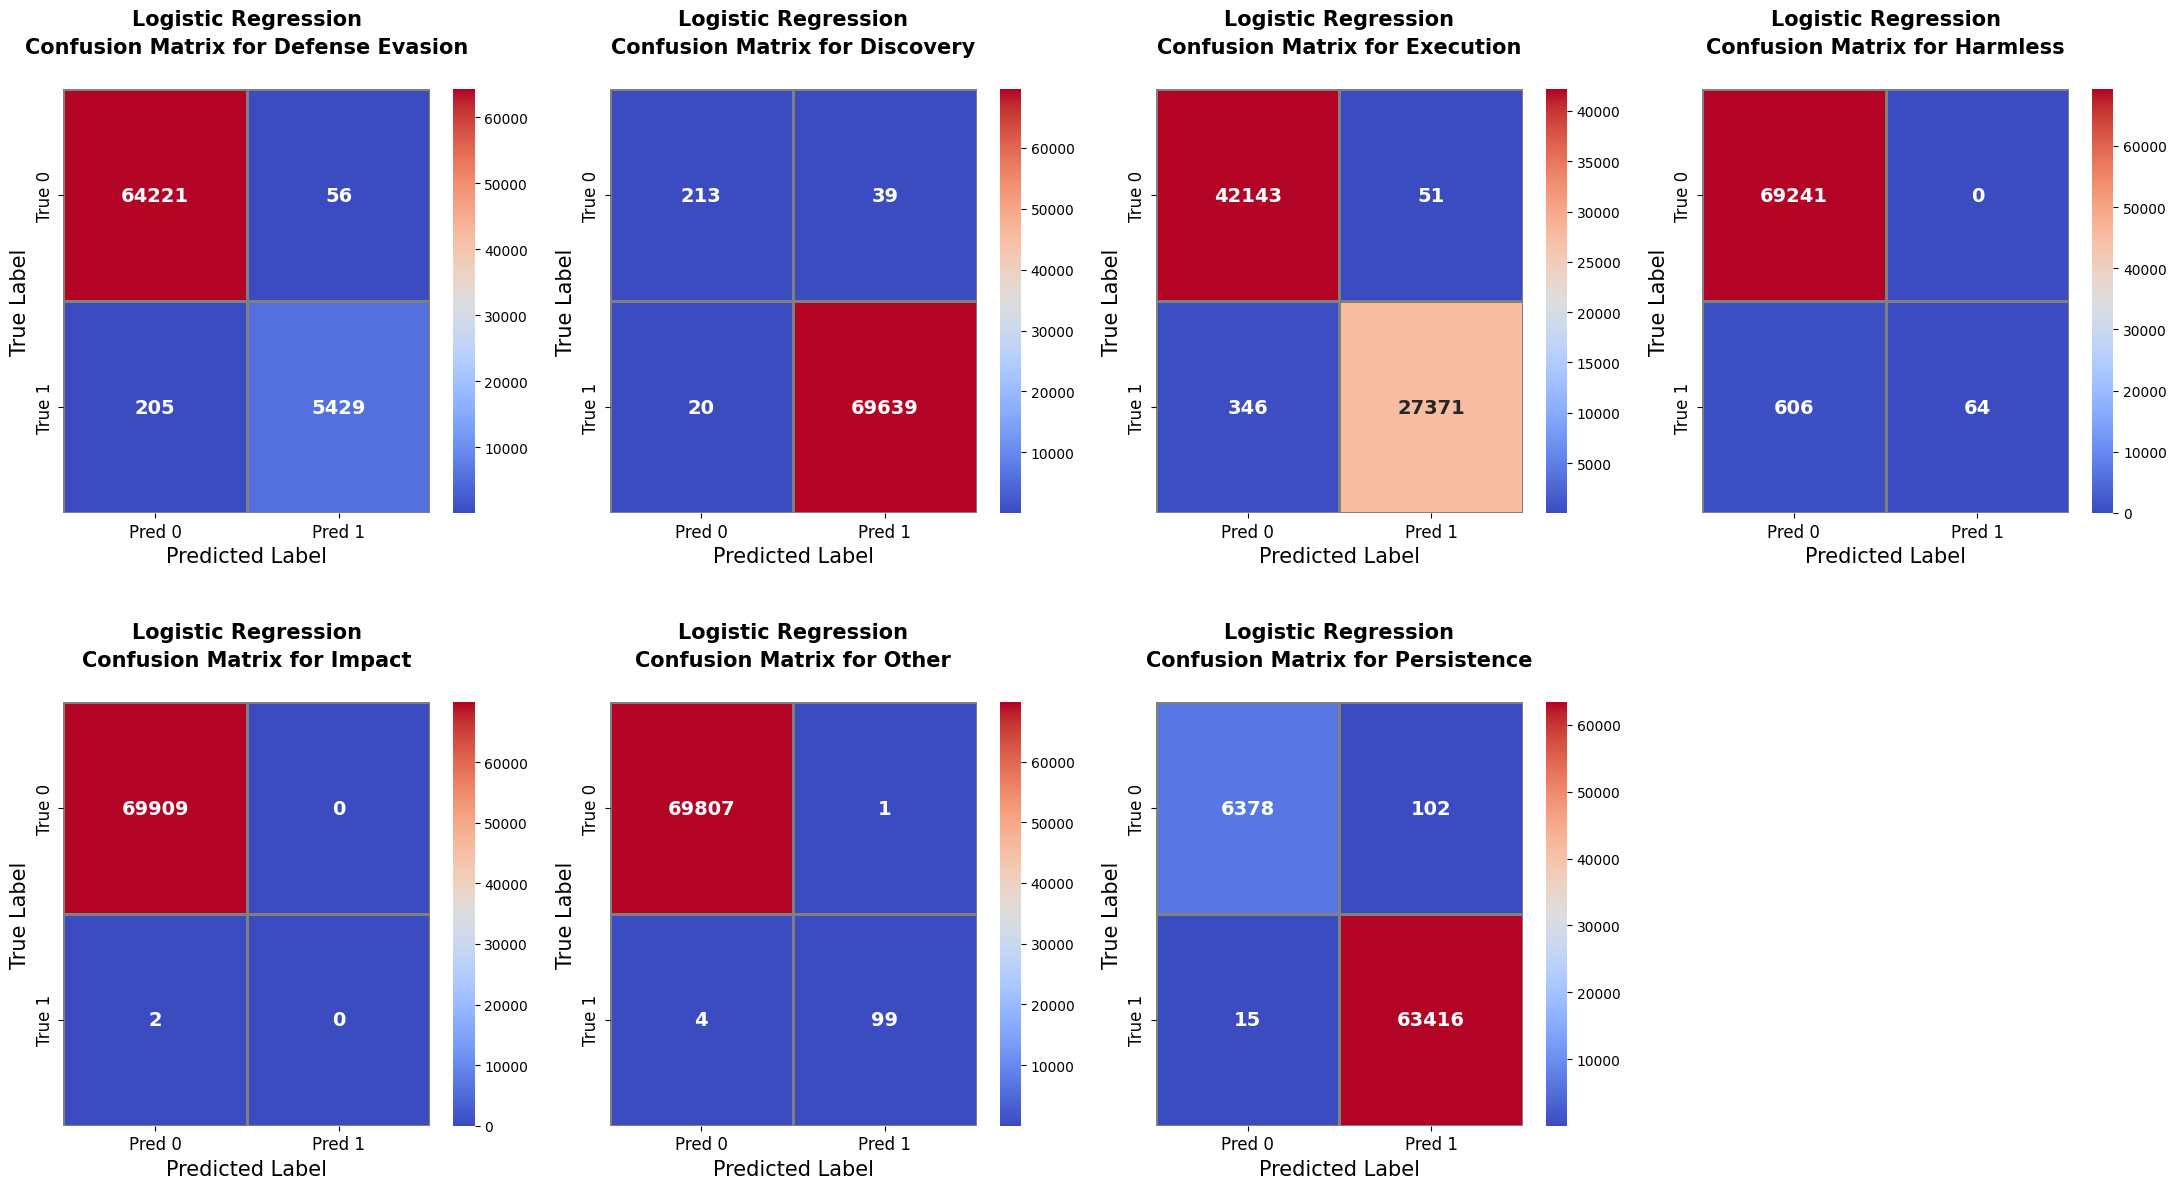
\includegraphics[width=0.9\textwidth]{../figures/plots/section2/Logistic_Regression_normalized_confusion_matrix_test.png}
                \caption{Confusion Matrix for Logistic Regression Model.}
                \label{fig:logistic_cm}
            \end{figure}

        \subsubsection{Hyperparameter Tuning \\}

            Grid search was performed to optimize the Logistic Regression model's hyperparameters. The search focused on varying the regularization parameter \( C \) over a range of values \([0.1, 1, 10, 100]\) to identify the configuration that maximized weighted F1-scores.

                \begin{lstlisting}[caption={Parameter grid for Logistic Regression}, label={lst:logistic_param_grid}]
                        # Define parameter grid for Logistic Regression
                        param_grid = {'C': [0.1, 1, 10, 100]}
                        grid_search = GridSearchCV(LogisticRegression(max_iter=1000, random_state=42), param_grid, cv=5)
                        grid_search.fit(X_train_tfidf, y_train_binary)
                \end{lstlisting}

            The optimized model exhibited improved performance compared to the baseline, particularly for intents with smaller sample sizes. Figure~\ref{fig:logistic_tuning} illustrates the weighted F1-scores for different values of \( C \).

            \begin{figure}[H]
                \centering
                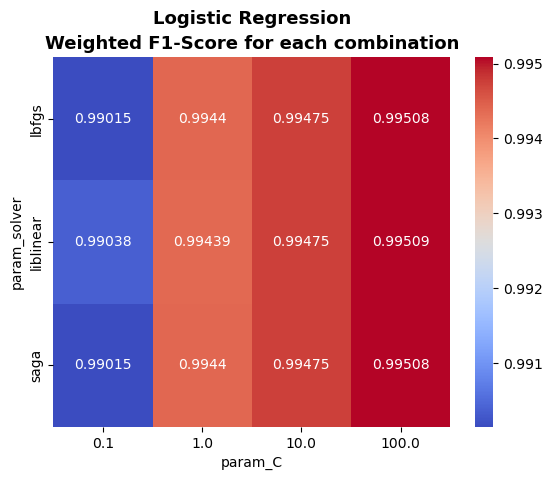
\includegraphics[width=0.9\textwidth]{../figures/plots/section2/weighted_f1_score_for_each_combination_of_parameters_logistic_regression.png}
                \caption{Weighted F1-Scores for Logistic Regression Hyperparameter Tuning.}
                \label{fig:logistic_tuning}
            \end{figure}

        \subsubsection{Comparative Analysis of Baseline and Optimized Models \\}

            The optimized Logistic Regression model demonstrated a moderate improvement in precision and recall compared to the baseline. However, its overall performance remained slightly inferior to more complex models like Random Forest and SVM. The comparative analysis underscores the importance of selecting models suited to the dataset's characteristics and problem requirements.

% 05-unsupervised-learning-clustering-appendix.tex

% Section Title
\section{UNSUPERVISED LEARNING - CLUSTERING}

    % Main Content
    
    \subsection{Impact of Data Preprocessing on Clustering Results} % TODO: update
    
        
    During our analysis, we experimented with different preprocessing techniques on the same dataset, leading to variations in cluster formations. Some preprocessing methods resulted in clearer separations, while others introduced more overlap between clusters. Given the interesting differences observed, we have included these visualizations in the appendix. We think that these visualizations could provide another perspective on the clustering results and help in understanding the impact of preprocessing on the clustering outcomes.
        
        \begin{figure}[h]
            \centering
            \begin{minipage}[c]{0.47\textwidth}
                \centering
                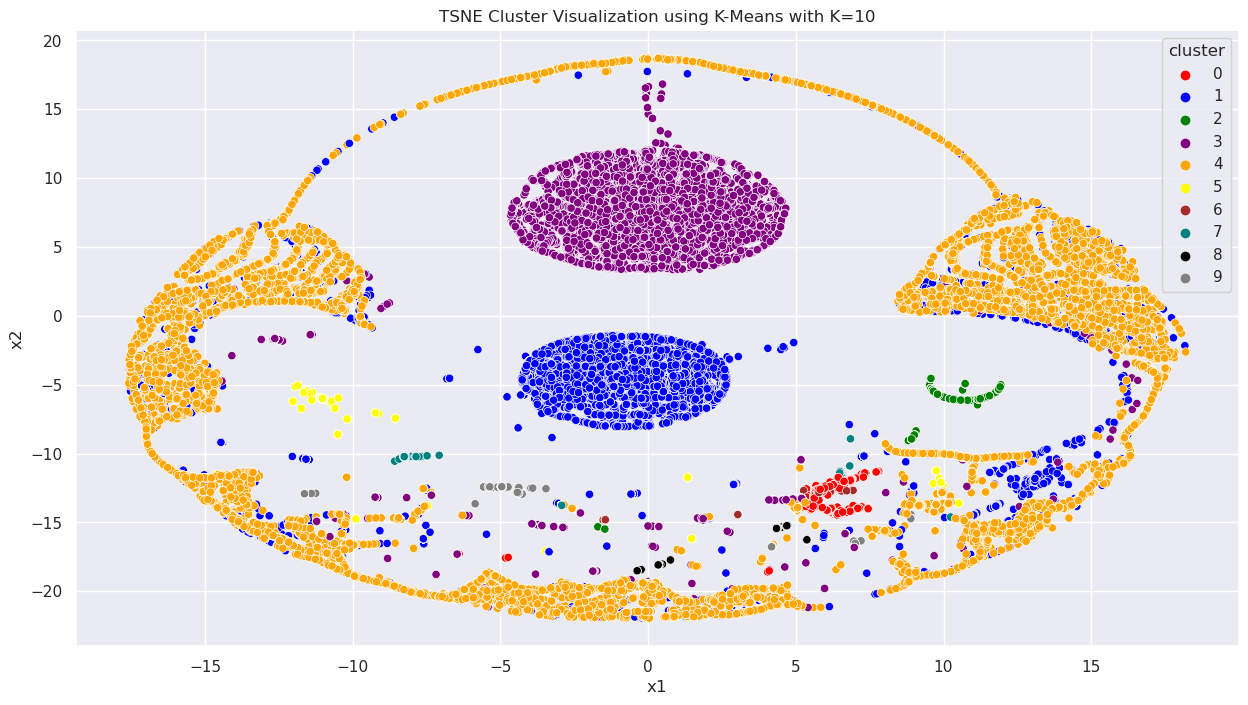
\includegraphics[width=\textwidth]{../figures/plots/section3/tsne_kmeans_clusters_1.png}
                \caption{t-SNE Visualization of K-Means Clusters}
                \label{fig:tsne_kmeans}
            \end{minipage}
            \hfill
            \begin{minipage}[c]{0.47\textwidth}
                \centering
                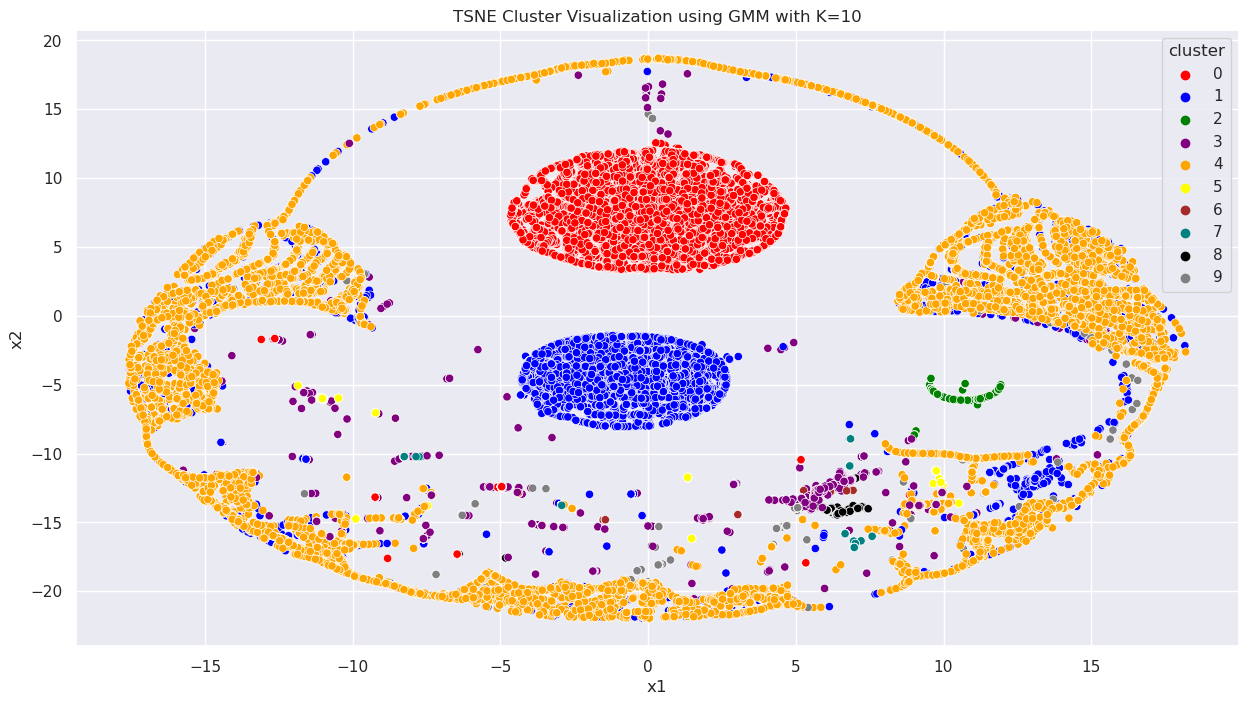
\includegraphics[width=\textwidth]{../figures/plots/section3/tsne_gmm_clusters_1.png}
                \caption{t-SNE Visualization of GMM Clusters}
                \label{fig:tsne_gmm}
            \end{minipage}
        \end{figure}
        
    \subsection{Intent distribution} % TODO: update
    
        The heatmaps illustrate the distribution of attack intents within the clusters formed by K-Means and GMM.
        
        \begin{figure}[h]
            \centering
            \begin{minipage}[c]{0.47\textwidth}
                \centering
                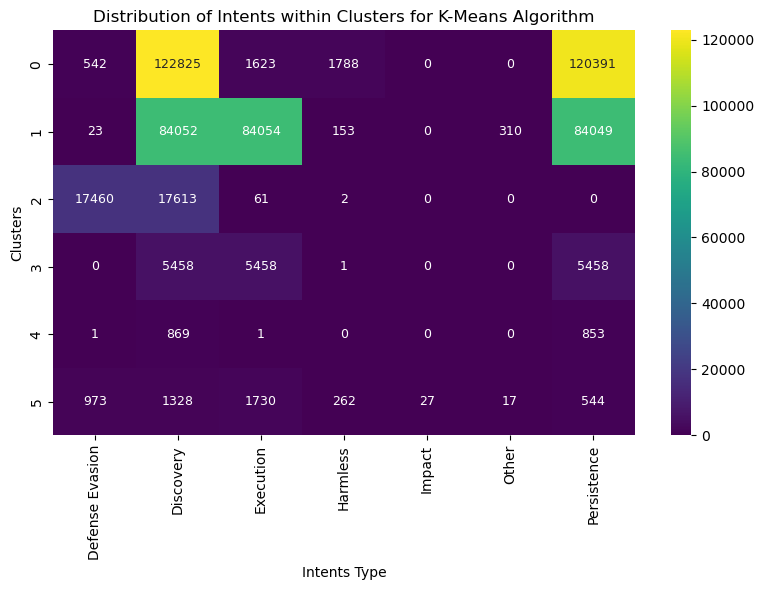
\includegraphics[width=\textwidth]{../figures/plots/section3/Intent_Distribution_kmeans.png}
                \vspace{-0.6cm}
                \caption{K-Means Intent Distribution}
                \label{fig:}
            \end{minipage}
            \hfill
            \begin{minipage}[c]{0.47\textwidth}
                \centering
                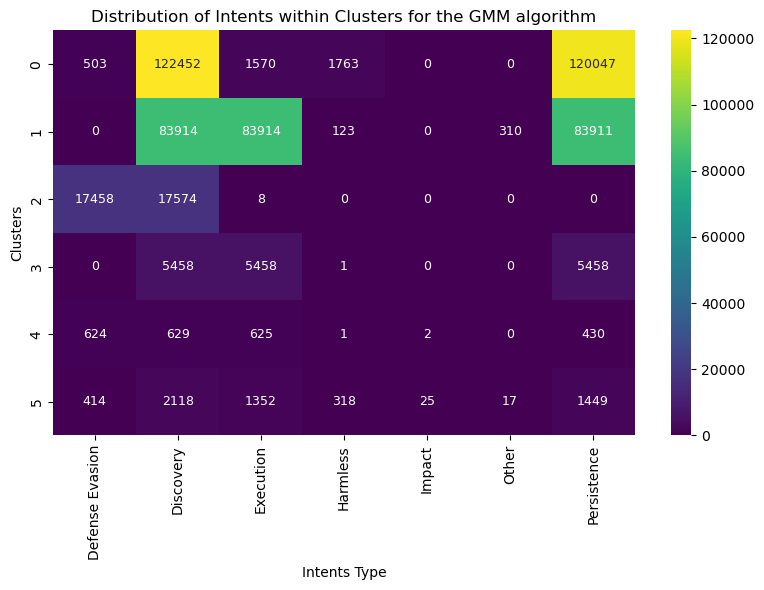
\includegraphics[width=\textwidth]{../figures/plots/section3/Intent_Distribution_gmm.png}
                \vspace{-0.6cm}
                \caption{GMM Intent Distribution}
                \label{fig:}
            \end{minipage}
        \end{figure}
    
% 06-language-model-exploration-appendix.tex

% Section Title
\section{LANGUAGE MODEL EXPLORATION}

    % Main Content
    
    \subsection{Training Configuration}

        The model was implemented using BERT (bert-base-uncased) with the following key configurations:
        \begin{itemize}
            \item Maximum sequence length: 128 tokens
            \item Learning rate: 4e-5 with AdamW optimizer ($\beta_1=0.9$, $\beta_2=0.98$, $\epsilon=1e-6$)
            \item Training epochs: 4
            \item Gradient accumulation steps: 4
            \item Mixed precision training enabled
            \item Linear learning rate scheduler without warmup
            \item Loss function: Binary Cross-Entropy with Logits
        \end{itemize}
        
    \subsection{Model Performance Metrics}

        \subsubsection{Class-wise F1 Scores}
        
            The model demonstrates varying performance across classes (Figure \ref{fig:f1_scores}):

            \begin{itemize}
                \item Excellent performance (F1 $\geq$ 0.98) for Defense Evasion, Discovery, Execution, Other, and Persistence classes
                \item Perfect scores (F1 = 1.00) for Discovery and Persistence
                \item Significantly lower performance for Harmless class (F1 = 0.22)
                \item Impact class shows minimal detection capability (F1 = 0.00)
            \end{itemize}

        \subsubsection{Detailed Performance Metrics}

            The performance metrics (Figure \ref{fig:performance_metrics}) reveal:

            \begin{itemize}
                \item Most classes achieve balanced precision and recall scores
                \item The Harmless class shows a significant disparity between precision and recall
                \item The Impact class shows minimal performance across all metrics
            \end{itemize}

        \subsubsection{Precision-Recall Analysis}

            The Precision-Recall curves (Figure \ref{fig:pr_curves}) demonstrate:

            \begin{itemize}
                \item Most classes maintain high precision (>0.95) across different recall thresholds
                \item The "Other" category shows a sharp decline in precision at approximately 0.2 recall
                \item Impact and Harmless classes demonstrate poor precision-recall trade-offs
                \item Defense Evasion, Discovery, Execution, and Persistence maintain near-perfect precision until very high recall values
            \end{itemize}

        \subsubsection{Prediction Probability Distribution}

            The prediction probability histograms (Figure \ref{fig:pred_prob}) reveal:

            \begin{itemize}
                \item Most classes exhibit a strong binary separation in prediction probabilities
                \item Defense Evasion, Discovery, and Execution show high-confidence predictions clustered near 0 and 1
                \item The Persistence class shows a similar pattern but with a smaller proportion of low-probability predictions
                \item Harmless and Impact classes show predominantly low-probability predictions, indicating potential class imbalance issues
            \end{itemize}
            
        \begin{figure}[h]
            \centering
            \begin{minipage}[c]{0.47\textwidth}
                \centering
                \vspace{0.1cm}
                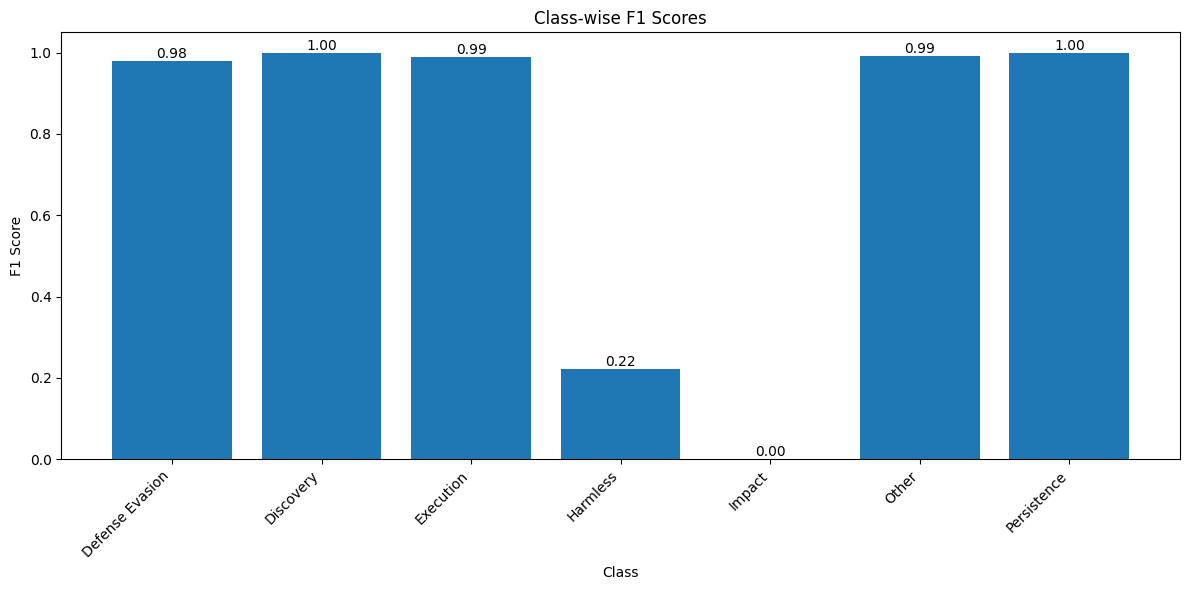
\includegraphics[width=\textwidth]{../figures/plots/section4/f1_scores.png}
                \caption{F1 scores across different classes showing the model's classification performance for each category.}
                \label{fig:f1_scores}
            \end{minipage}
            \hfill
            \begin{minipage}[c]{0.47\textwidth}
                \centering
                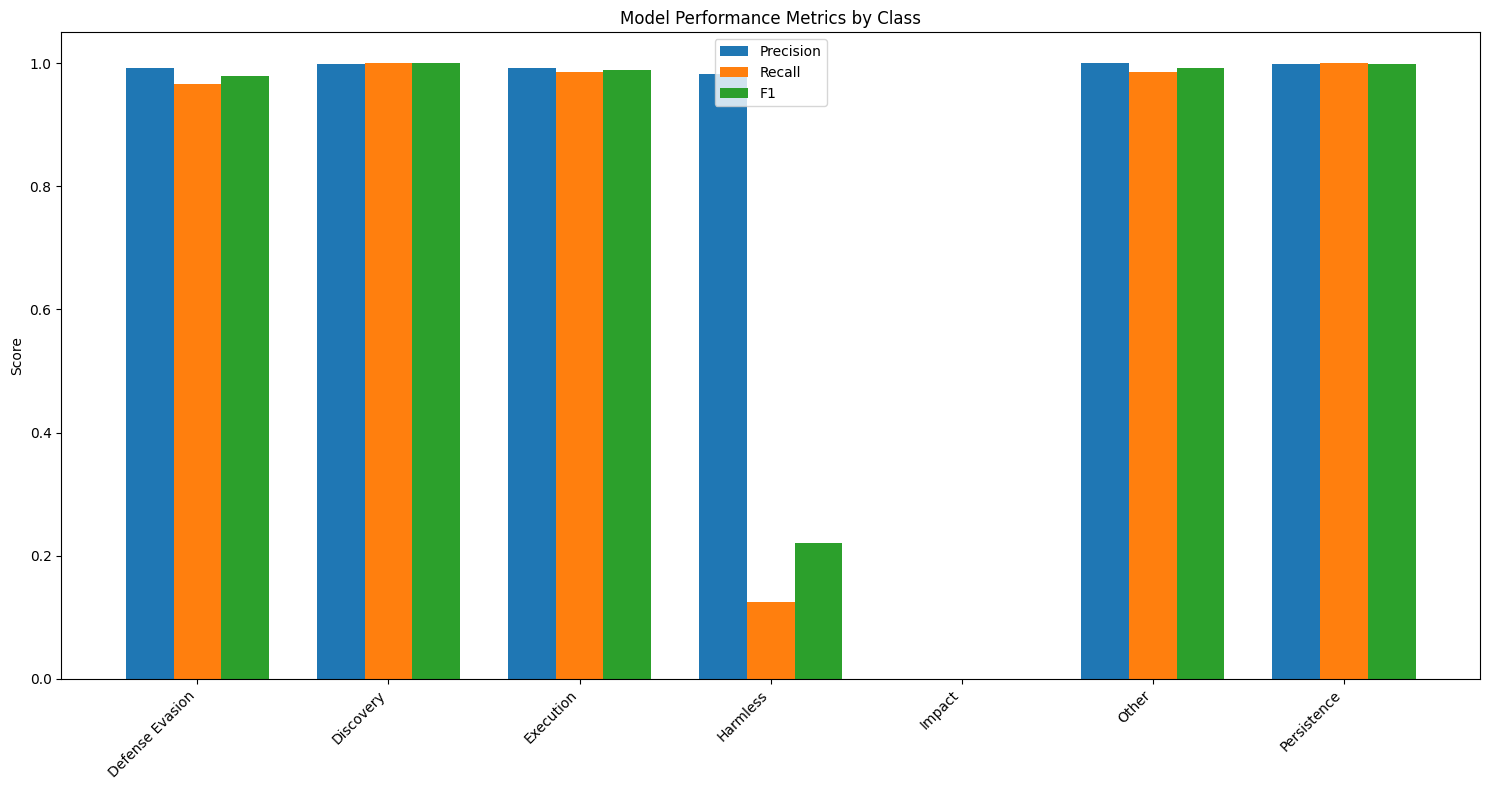
\includegraphics[width=\textwidth]{../figures/plots/section4/performance_metrics.png}
                \caption{Detailed breakdown of Precision, Recall, and F1 scores for each class.}
                \label{fig:performance_metrics}
            \end{minipage}
        \end{figure}
        
        \begin{figure}[h]
            \centering
            \begin{minipage}[c]{0.47\textwidth}
                \centering
                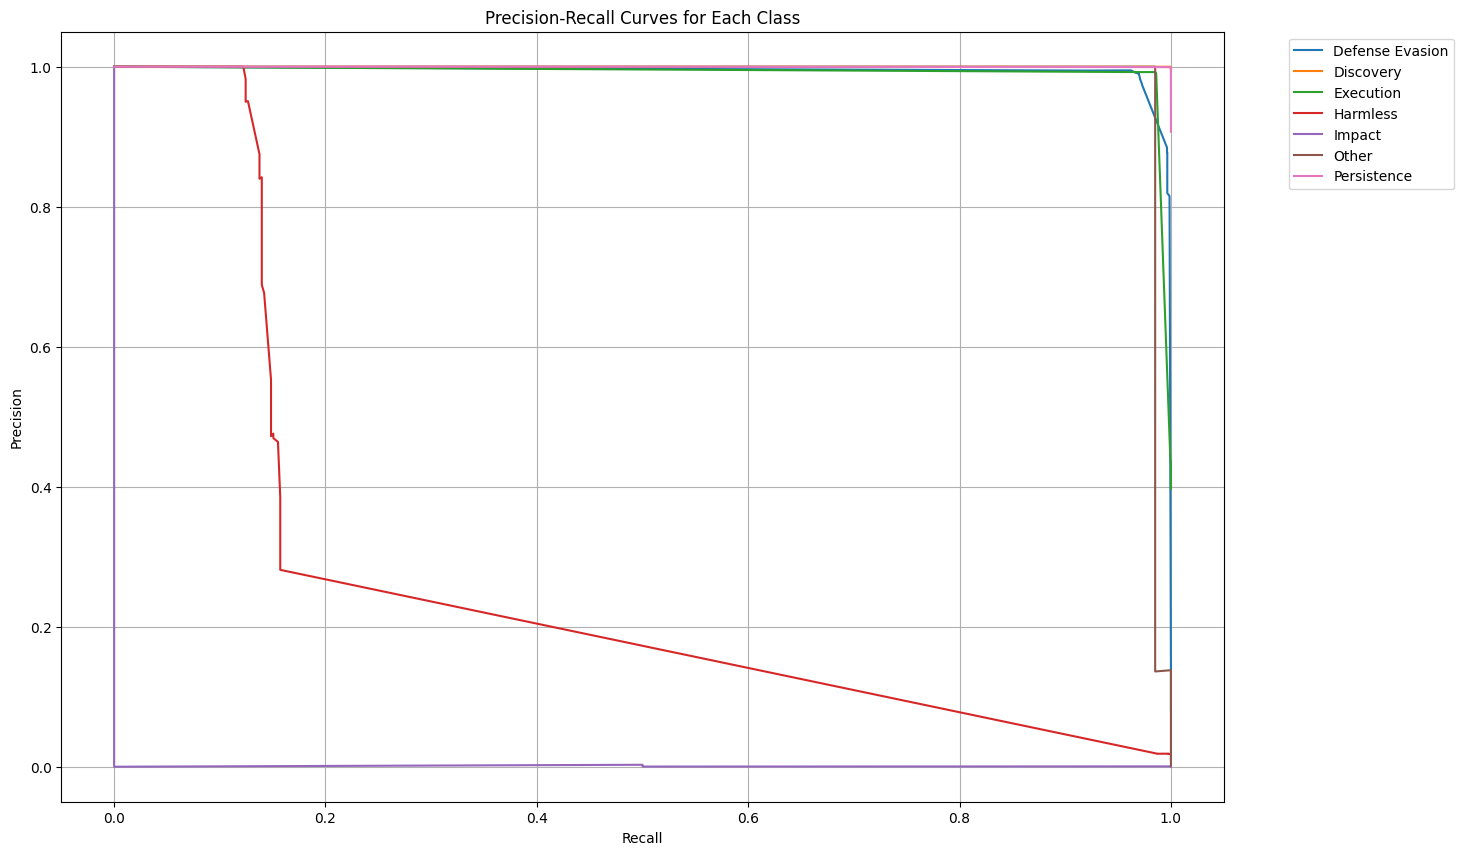
\includegraphics[width=\textwidth]{../figures/plots/section4/precision_recall_curves.png}
                \caption{Precision-Recall curves for each class showing the trade-off between precision and recall at different classification thresholds.}
                \label{fig:pr_curves}
            \end{minipage}
            \hfill
            \begin{minipage}[c]{0.47\textwidth}
                \centering
                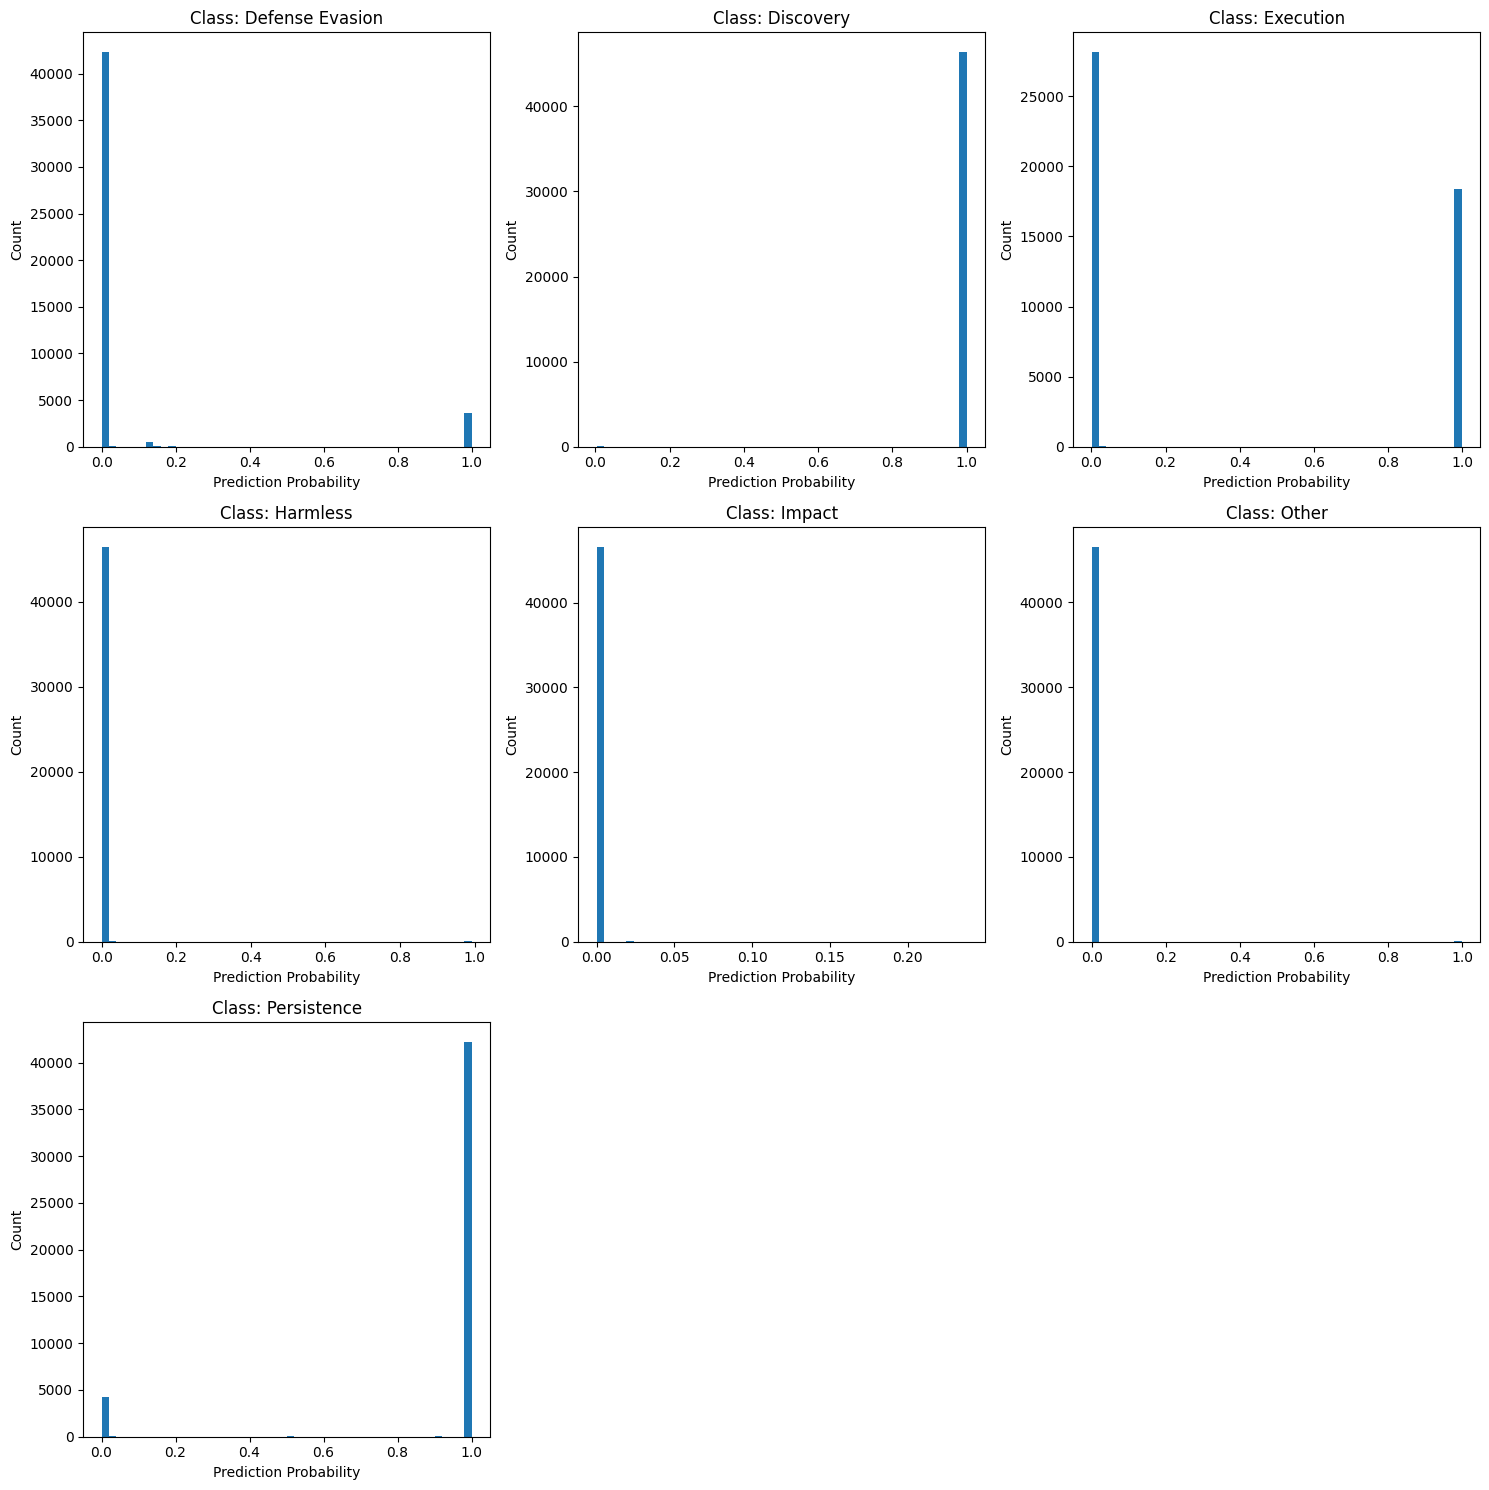
\includegraphics[width=0.7\textwidth]{../figures/plots/section4/probability_histograms.png}
                \caption{Distribution of prediction probabilities for each class showing the model's confidence in its predictions.}
                \label{fig:pred_prob} 
            \end{minipage}
        \end{figure}
        
        
    \subsection{Recommendations for Model Improvement}

        Based on the analysis, several potential improvements could be considered:

        \subsubsection{Class Imbalance Mitigation}
        
            \begin{itemize}
                \item Implement class weights or sampling techniques for Harmless and Impact classes
                \item Consider data augmentation for underrepresented classes
            \end{itemize}

        \subsubsection{Model Architecture}
        
            \begin{itemize}
                \item Experiment with different BERT variants
                \item Consider ensemble approaches for improving performance on challenging classes
            \end{itemize}

        \subsubsection{Training Strategy}
        
            \begin{itemize}
                \item Implement curriculum learning for difficult classes
                \item Explore different learning rate schedules
                \item Consider longer training with early stopping
            \end{itemize}

        \subsubsection{Data Quality}
        
            \begin{itemize}
                \item Review and potentially relabel samples in the Impact class
                \item Analyze misclassified examples in the Harmless class
            \end{itemize}
    

% TODO: check
% Include the bibliography file
\bibliography{../template/column-format-template/sample-base}

% At end of document
% \bibliography{references}           % Single .bib file
% \bibliography{ref1,ref2,ref3}       % Multiple .bib files

\end{document}
